\documentclass{SBCbookchapter}
\usepackage[utf8]{inputenc}
\usepackage[T1]{fontenc}
\usepackage[brazil,english]{babel}
\usepackage{graphicx}
\title{Typhoon Classification: An Ensemble Machine Learning Approach}
\begin{document}
\maketitle

%\addcontentsline{toc}{chapter}{Statistics}

%\emph{Find a statistical method which uses only Japan Meteorological Agency (JMA) best track typhoon data during or before year $n$ to hind-cast the entire best track of all typhoons in years $n+1$.   Given only the latter typhoons' initial three best track points (i.e. at $t=0,6,$ and $12$ hours), the maximum position error at each hind-casted track point must be less than 500 km. The method must work for the three most recent years of published best track data.}

\vspace{.3in}
\begin{minipage}[r]{4.25in}{\small
  The enormous devastation caused by super typhoon Haiyan (2013) motivates us to consider whether data from past typhoons hold a key to predicting the grade (``category'') of an emerging tropical storm from early best track data (lat, lon, windspeed and pressure in the first 18 hours). In particular, we describe the ensemble approach to machine learning (ML) classification and the utilize MATLAB's Machine Learning Toolbox to create an ensemble based model prediction script. We train the mdoel using 2009-2014 best-track data and validate it using 2015 data.}
\end{minipage}

\newpage

\section{Introduction}

  In November 2013, Typhoon Haiyan struck the Philippines with sustained wind speeds of nearly 200
miles per hour, claiming over 6,000 lives, displacing 4 million people, damaging over a million houses,
and resulting in a request for over 750 million dollars
in humanitarian aid. Devastation caused by
``super typhoons" like Haiyan makes the on-going
development of early warning systems an absolute
necessity to provide vulnerable communities sufficient preparation time to
mitigate damage to both life and property. This motivates us to apply Machine Learning algorithms to predict th Machine Learning category, wind speed and location of emerging typhoons.

\section{Supervised Machine Learning}

Supervised Machine learning (ML) utilizes a training data set to develop a model which includes one or more input variables called \emph{predictors} and outputs the value of a variable called a \emph{response}.  For example, our predictors might be data for  the lat, lon, pressure and windspeed of an emerging tropical storm, and response might be the grade of the typhoon (3,4, or 5) or its  maximum wind (any value  35 km/hr or greater).  When the response is a discrete set, such as is the case for typhoon grade, we use a \emph{categorical} SML algorithm. When the response is continuous, such as maximum wind speed, we use a \emph{regression} algorithm.  In this lab, we do not consider \emph{unsupervised} ML algorithms where the response variables are not known in advance, and hence not specified in the training data set.  

Once a model has been developed using the training data set, it can be validated using a \emph{validation} data set. 
A validated model can then be used for new data

In our case, we will use Japan Meteorological Agency (JMA) data for 2009-2014 as training data:

\begin{itemize}
\item Predictor Variables: Lat, Lon, WS and Pressure at times $t=0,6,12,18$ hours.
\item Response Variables: Grade, maximum wind speed.
\end{itemize}
{\flushleft We use} JMA data for 2015-2016 as our validation set.  For a quasi-operational (``hind-casting") model, our "new" data is JMA data for 2017.


There are a number of basic supervised ML algorithms \cite{Bon} such as

\begin{itemize}
    \item Decision Tree 
    \item Support Vector Machines (SVM)
    \item K nearest neighbors
    \item Ensemble
\end{itemize}

{\flushleft In} this chapter, we consider the ensemble approach.

\section{Ensemble Classification}
Predicting the JMA grade of an emerging tropical storm based on its initial 18 hour bext track data is an example of a standard supervised learning problem (\cite{Diet}).  Given training data of the form $\{({\bf x}_1,y_1),...,({\bf x}_m,y_m)$  where ${\bf x_.}=(YEAR,MONTH,DAY,LAT1,LON1,PRES1,WS1,LAT2,LON2,PRES2,WS2,LAT3,LON3,PRES3,WS3,LAT4,	LON4,PRES4,WS4)$ specifies the date and first three best track points of an emerging tropical storm (recorded winspeed of 35 knots).

\section{MATLAB's ML Toolbox}
Using MATLAB's classification app (included in the Statistics and Machine Learning Toolbox) the confusion matrix (Figure \ref{fig1}) indicates that 47 Grade 5 typhoons are correctly predicted, with 13 false positive (8 Grad 4 and 5 Grade 3) and 16 False Negative (7 predicted as Grade 3 and 9 as Grade 4).  

 \begin{figure}[!htpb]
 \centering
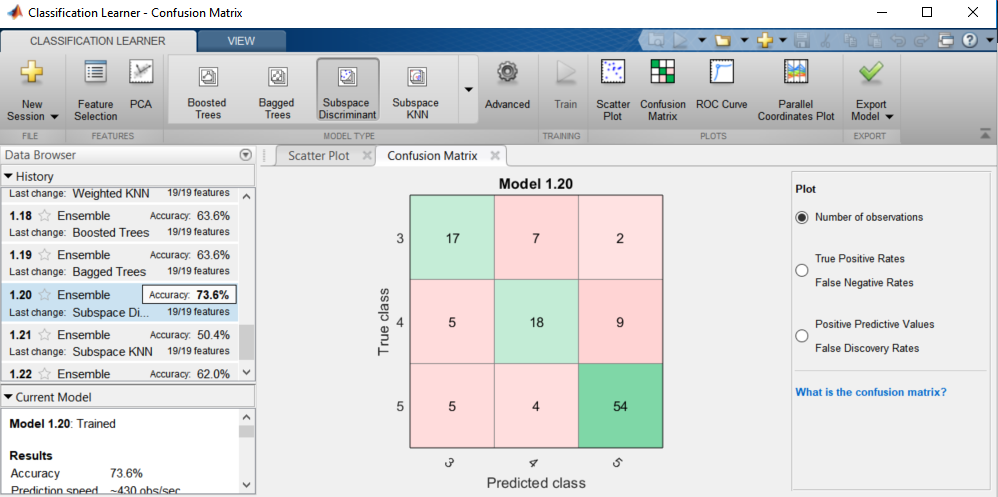
\includegraphics[width=3in,height=1.75in]{Ensemblefig1.png}
\caption{Confusion matrix for MATLAB's Subspace Discriminant Ensemble classification algorithm (73.6\% Accuracy) }
\label{fig1}
\end{figure}

\vspace{.25in}

The Fine Tree algorithm regerssion plot (Figure \ref{fig2}) shows fairly good wind speed prediction of Grade 5 violent typhoon (maximum wind speeds of at least 105 knots/hr).

 \begin{figure}[!htpb]
 \centering
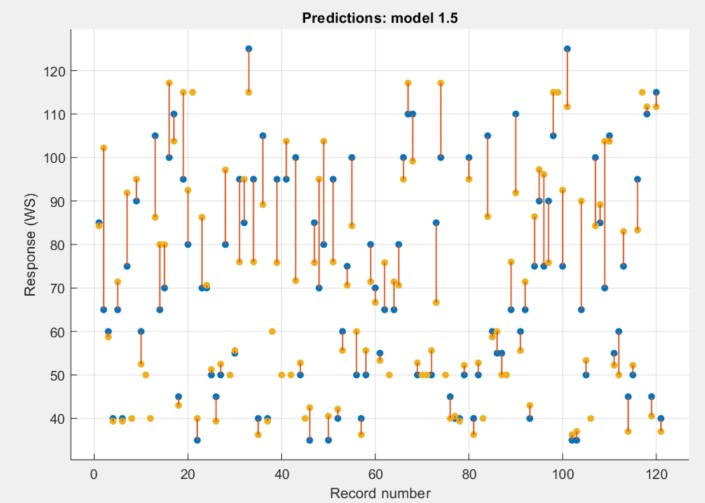
\includegraphics[width=3in,height=1.75in]{TyphoonCM2.png}
\caption{MATLAB's Fine Tree regression model RMSE: 11.0 }
\label{fig2}
\end{figure}

\section{Assignment}https://www.overleaf.com/project/5c057323a87843644f4893a6


\section{Computer Project}
\begin{enumerate}
\item Using the same training and validation data sets, use MATLAB to create 
an ensemble based regression model for the highest wind speed attained on a best track.
\end{enumerate}

\emph{Project Team:} Michaela Flitsch, Mark Nussbaum, Zach Oslund, Matthew Rueger.

\newpage
 \begin{thebibliography}{9}

 \bibitem{Bon}  {Bonnardot, G.}, 8 Machine Learning Algorithms Explained in Human Language. Available at https://www.datakeen.co/en/8-machine-learning-algorithms-explained-in-human-language/
 
 \bibitem{Diet} {Dietterich, T.} Ensemble Methods in Machine Learning.  Available at http://web.engr.oregonstate.edu/~tgd/publications/mcs-ensembles.pdf
 
\bibitem{JMA} {Japan Meteorological Agency},  Best track archives. Available at  http://www.jma.go.jp/ jma/jma-eng/ jma-center/ rsmc-hp-pub-eg/trackarchives.html.

\end{thebibliography}
\end{document}
%
%\item Japan Meteorological Agency, 2014: {\em Annual Report of the RSMC Tokyo-Typhoon Center 2013}. http://www.jma.go.jp/jma/ jma- eng/jma-center/rsmc-hp-pub-eg/AnnualReport/2013/Text/Text2013.pdf
%
%
%\item Jin, L., C. Yao and X. Huang, 2008: A Nonlinear Artificial Intelligence Ensemble Prediction Model for Typhoon Intensity. \emph{Mon. Weather Rev.}, {\bf 136}, 4541-4554.
%
%\item Knaff, J.A., C.R. Sampson, and M. DeMaria, 2005: An operational statistical intensity prediction scheme for the western north Pacific. \emph{Weather Forecast.}, {\bf 20}, 688-699.
%
%
%    \item Komaromi, W.A., S.J. Majumdar and E.D. Rappin, 2011: Diagnosing initial condition sensitivity of typhoon Sinlaku (2008) and hurricane Ike (2008), {\bf 139}, 3224-3241.
%
%\item  Korean Meteorological Administration, 2013: {\em Annual Report}. \\ http://web.kma.go.kr/download\_01/Annual\_Report\_2013.pdf
%
%\item Krishnamurti, T.N., J. Xue, H.S. Bedi, K. Ingles, and D. Oosterhof, 1991: Physical initialization for numerical weather prediction over the tropics. \emph{Tellus}, {\bf 43}, 53-81.
%
%\item Krishnamurti, T.N., C.M. Kishtawal, T.E. LaRow, D.R. Bachiochi, Z. Zhang, C.E. Williford, S. Gadgil, and S. Surendran, 1999: Improved weather and seasonal climate forecast from multi-model superensemble. \emph{Science}, {\bf 285}, 1548-1550.
%
%\item Leith, C.E., 1974: Theoretical skill of Monte-Carlo forecasts. \emph{Mon. Wea. Rev.,} {\bf 102}, 409-418.
%
%\item Leslie, L.M., R. Abbey and G.J. Holland, 1998. Tropical cyclone track predictability. \emph{Meteorol. Atmos. Phys.}, {bf 65}, 223-231.
%
%\item Lorenz, E.N., 1963: Deterministic nonperiodic flow. \emph{J. Atmos. Sci.}, {\bf 20}, 130-142.
%\item Lorentz, E.N., 1965: A study of the predictability of a 28-variable atmospheric model. \emph{Tells}, {\bf 17}, 321-333.
%
%\item Meng, Z. and F. Zhang, 2007: Tests of an ensemble Kalman filter for mesoscale and regional-scale data assimilation. Part II: Imperfect model experiments. \emph{Mon. Weather Rev.,} {\bf 135}, 1403-1423.
%
%\item Neumann, C. J., 1972: An alternate to the HURRAN tropical cyclone forecast system. \emph{NOAA Tech. Memo.} NWS SR-62, 22 pp.
%
%\item  Rozanova, O. S., J.-L. Yu, and C.-K. Hu, 2010: Typhoon eye trajectory based on a mathematical model: comparing
%with observational data. \emph{Nonlinear Analysis: Real World Applications.} {\bf 11}, 1847�1861.
%
%\item $\ddot{\textup{U}}$ster, H. and R.F. Love, 2001: Application of a weighted sum of order $p$ to distance estimation. \emph{IIE Trans.}, {\bf 33}, 675-684.
%
%\item Weber, H., 2005: Probabilistic prediction of tropical cyclones. part 1: position. \emph{Mon. Weather Rev.}, {\bf 133}, 1840-1852.
%
%\item Williford, C.E., T.N. Krishnamurti, R.C. Torres, and S. Cocke, 2003: Real-time multimodel superensemble forecasts of Atlantic tropical systems of 1999. \emph{Mon. Weather Rev.}, {\bf 131}, 1878-1894.
%
%\item Wu, C.-C., and K. Emmanuel, 1993: Interaction of baroclinic vortex with background shear: application to hurricane movement. \emph{J. Atmos. Sci.}, {\bf 50}, 62-76.
%
%    \item Yamaguchi, M., T. Nakazawa, and K. Aonashi, 2012:  Tropical Cyclone track forecasts using JMA model with ECMWF and JMA initial conditions. \emph{Geophys. Rev. Lett.,} {\bf 39}, L09801, doi:10.1029/2012GL051473.
%
%\item Yanase, W., H. Taniguchi, M. Satoh, 2010: The genesis of tropical cyclone Nargis (2008): environmental modulation and numerical probability. \emph{J. Meteor. Soc. of Japan}, {\bf 88}, 407-519.
%
%        \item Yang, S.-C., E. Kalnay and T. Miyoshi, 2012: Accelerating the EnKF spinup for typhoon assimilation and prediction. \emph{Weather Forecast.}, {\bf 27}, 878-897.
%
%\end{list}

%Official annual tropical storm and typhoon best track data (lat, lon, windspeed, pressure in 6 hour time increments) is published by the Japan Meteorological Agency (JMA). To develop a best track prediction model, you are allowed to use as your training data the JMA best track data for the thirteen typhoons Soulik, Utor, Manyi, Usagi, Wutip, Fitow, Dana, Nari, Wipha, Francisco, Lekima, Krosa, and Haiyan in 2013  available at
%  \\ {\scriptsize http://www.jma.go.jp/jma/jma-eng/jma-center/rsmc-hp-pub-eg/besttrack.html}.
%{\flushleft Design} a model such that given just the 2013 training data and the initial best track point of the eleven typhoons in 2014 shown in the table below, you can predict the best track position of each 2014 typhoon at the 120 hour mark with an average error of less than 500 km.
%
%\begin{table}[!htpb]
%\scriptsize
%\centering
%\begin{tabular}{|c|l||c|c|c|c|}\hline
% Typhoon& International&\multicolumn{4}{|c|}{Initial best track}\\
%        & I.D. &lat & lon & pressure  & wind speed\\\hline
% Faxai&1403&8.7&147.8&1004&0\\\hline
% Neoguri& 1408&8.4&146.8&1006&0\\\hline
% Rammasun &1409&8.0&154.3  &1006&0\\\hline
% Matmo& 1410&10.0&136.8&1006&0\\\hline
% Halong  & 1411&11.3 &151.8& 1006&0\\\hline
% Genevieve  & 1413&13.6 &181.2& 950&0\\\hline
% Kalmaegi&1415&13.5 &134.0&1004&0\\\hline
% Phanfone   & 1418 &11.0& 157.1&1004&0\\\hline
% Vongfong &  1419&7.3 &162.1&1006&0\\\hline
% Nuri & 1420&12.6 & 140.9&1004&0\\\hline
% Hagupit& 1422&2.6&156.0&1006&0\\\hline\hline
%  \end{tabular}
%  \caption{ Initial best track points of typhoons in 2014.}
%  \end{table}
%
%\vspace{.3in}
%
%
\end{document}